Conservation of invariants. Consider the following model of a chemical reaction:
\begin{align*}
	\dot x_1 &= -0.04\,x_1 + 10^4\,x_2\,x_3,\\
	\dot x_2 &= 0.04\,x_1 - 10^4\,x_2\,x_3 - 3\cdot 10^7\,x_2^2,\\
	\dot x_3 &= 3\cdot 10^7\,x_2^2,
\end{align*}
with the initial conditions:
\begin{align*}
	x_1(0) &= 1, & x_2(0) &= 2\cdot 10^{-4}, & x_3(0) &= 3\cdot10^{-1}
\end{align*}
\begin{enumerate}
	\item[(a)] Show that mass conservation $x_1(t)+x_2(t)+x_3(t) = x_1(0)+x_2(0)+x_3(0) =  M$ is an invariant for the model.
	
	Mass conversation $\implies \dot x_1(t)+\dot x_2(t)+\dot x_3(t) = 0$. \\
	Let the coefficients of $x_1(t),\ x_2(t)\,x_3(t),\ x_2^2(t)$ be $p_1,\ p_2,\ p_3$, respectively. \\
	Then, 
	\begin{align*}
		\dot x_1(t)+\dot x_2(t)+\dot x_3(t) &= -p_1\,x_1 + p_2\, x_2\,x_3 + p_1\,x_1 - p_2\,x_2\,x_3 - p_3\,x_2^2 + p_3\,x_2^2 = 0\\
	\end{align*}
	where, 
	\begin{align*}
		p_1 &= 0.04, & p_2 &= 10^4, & p_3 &= 3\,10^7. 
	\end{align*}*
	Integrating, $\dot x_1(t)+\dot x_2(t)+\dot x_3(t)$, we get: 
	\begin{align*}
		\int \dot x_1(t)+\dot x_2(t)+\dot x_3(t) &= x_1(t) + x_1(0) + x_2(t) + x_2(0) + x_3(t) + x_3(0) = 0\\
		x_1(t) + x_2(t) + x_3(t) &= -(x_1(0) + x_2(0) + x_3(0)) = M
	\end{align*}
	i.e. $x_1(t) + x_2(t) + x_3(t)$ is invariant.
	\item[(b)] The invariant is a linear first integral
	A linear first integral is of teh form:
	\begin{align*}
		c + b^T\,X.
	\end{align*}
	Here,
	\begin{align*}
		X &= [x_1\ x_2\ x_3], & b = []
	\end{align*}
	\item[(c)] Conservation of linear first integrals
	
	The model was simulated in Matlab using \texttt{ode45} RK4-5 solver.
	
	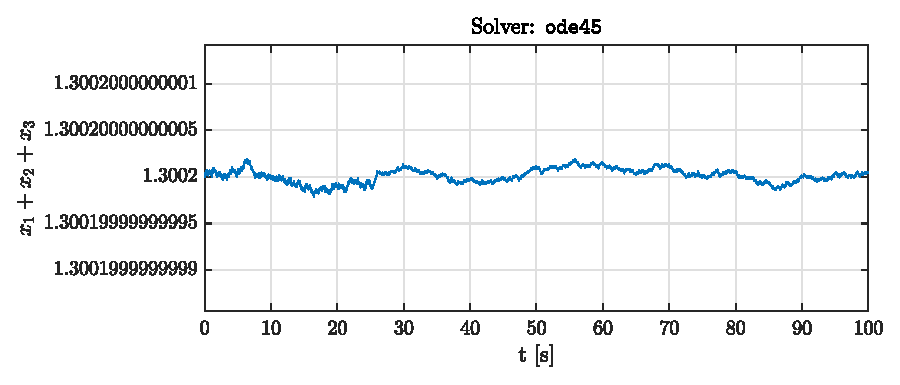
\includegraphics[width=\textwidth]{Figures/Ugf18c.eps}
	
	From the above figure it is clear that the solver  conservers the linear first integral.
	
	\item[(d)] Conservation of quadratic integrals
	The "circle drawer" is given by the following:
	\begin{align*}
		\dot y_1 &= -y_2, & \dot y_2 &= y_1, \\
		y_1(0) &= 1, & y_2(0) &= 0,
	\end{align*}
	The model was simulated in Matlab using \texttt{ode45} RK4-5 solver. The quadratic invariant is given as $y_1^2 + y_2^2$. 
	
	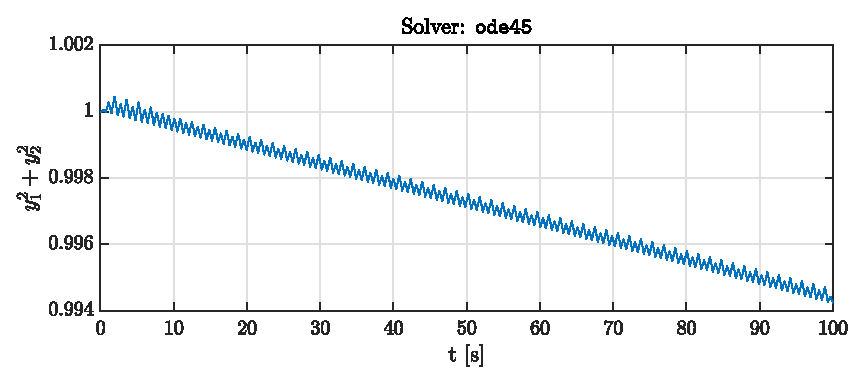
\includegraphics[width=\textwidth]{Figures/Ugf18d.eps}
	
	The above figure presents the quadratic invariant and it is clear that the RK4-5 method does not keep the invariant.
\end{enumerate}